\section{Потенциальное движение}
\label{sec:p9}

Из закона сохранения циркуляции скорости можно вывести важное следствие. Будем
считать сначала, что движение жидкости стационарно и рассмотрим линию тока, о
которой известно, что в некоторой ее точке $\rot\vv = 0$. Проведем бесконечно
малый контур, охватывающий линию тока вокруг этой точки; с течением времени он
будет передвигаться вместе с жидкостью, все время охватывая собой ту же самую
линию тока. Из постоянства произведения (\ref{eq:8.2}) следует поэтому, что $\rot\vv = 0$
будет равен нулю вдоль всей линии тока.

Таким образом, если в какой-либо точке линии тока завихренность отсутствует, то
она отсутствует и вдоль всей этой линии. Если движение жидкости не стационарно,
то этот результат остается в силе, с той разчицей, что надо говорить не о линии
тока, а о траектории, описываемой с течением времени некоторой определенной
жидкой частицей (напоминаем, что при нестационарном движении эти траектории не
совпадают, вообще говоря, с линиями тока) \footnote{Во избежании недоразумений
отметим уже здесь, что этот результат теряет смысл при турбулентном движении.
Отметим также, что завихренность может появиться на линии тока после пересечения
ею так называемой ударной волны; мы увидим, что это связано с нарушением изэнтропичности
течения (\S\ref{sec:p114})}.

На первый взгляд отсюда можно было бы сделать следующий вывод. Рассмотрим
стационарное обтекание какого-либо тела потоком жидкости. На бесконечности
натекающий поток однороден; его скорость $\vv = \const$, так что $\rot\vv \equiv
 0$ на всех линиях тока. Отсюда можно было бы заключить, $\rot\vv$ будет равен
нулю и вдоль всей длины всех линий тока, т. е. во всем пространстве.

Движение жидкости, при котором во всем пространстве $\rot\vv = 0$, называется
потенциальным (или безвихревым) в противоположность вихревому движению, при
котором ротор скорости отличен от нуля. Таким образом, мы пришли бы к
результату, что стационарное обтекание всякого тела натекающим из бесконечности
однородным потоком должно быть потенциальным.

\begin{wrapfigure}{r}{6cm}
% "l" or "r" for the side on the page.
% And the width parameter for the width of the image space.
  \centering
  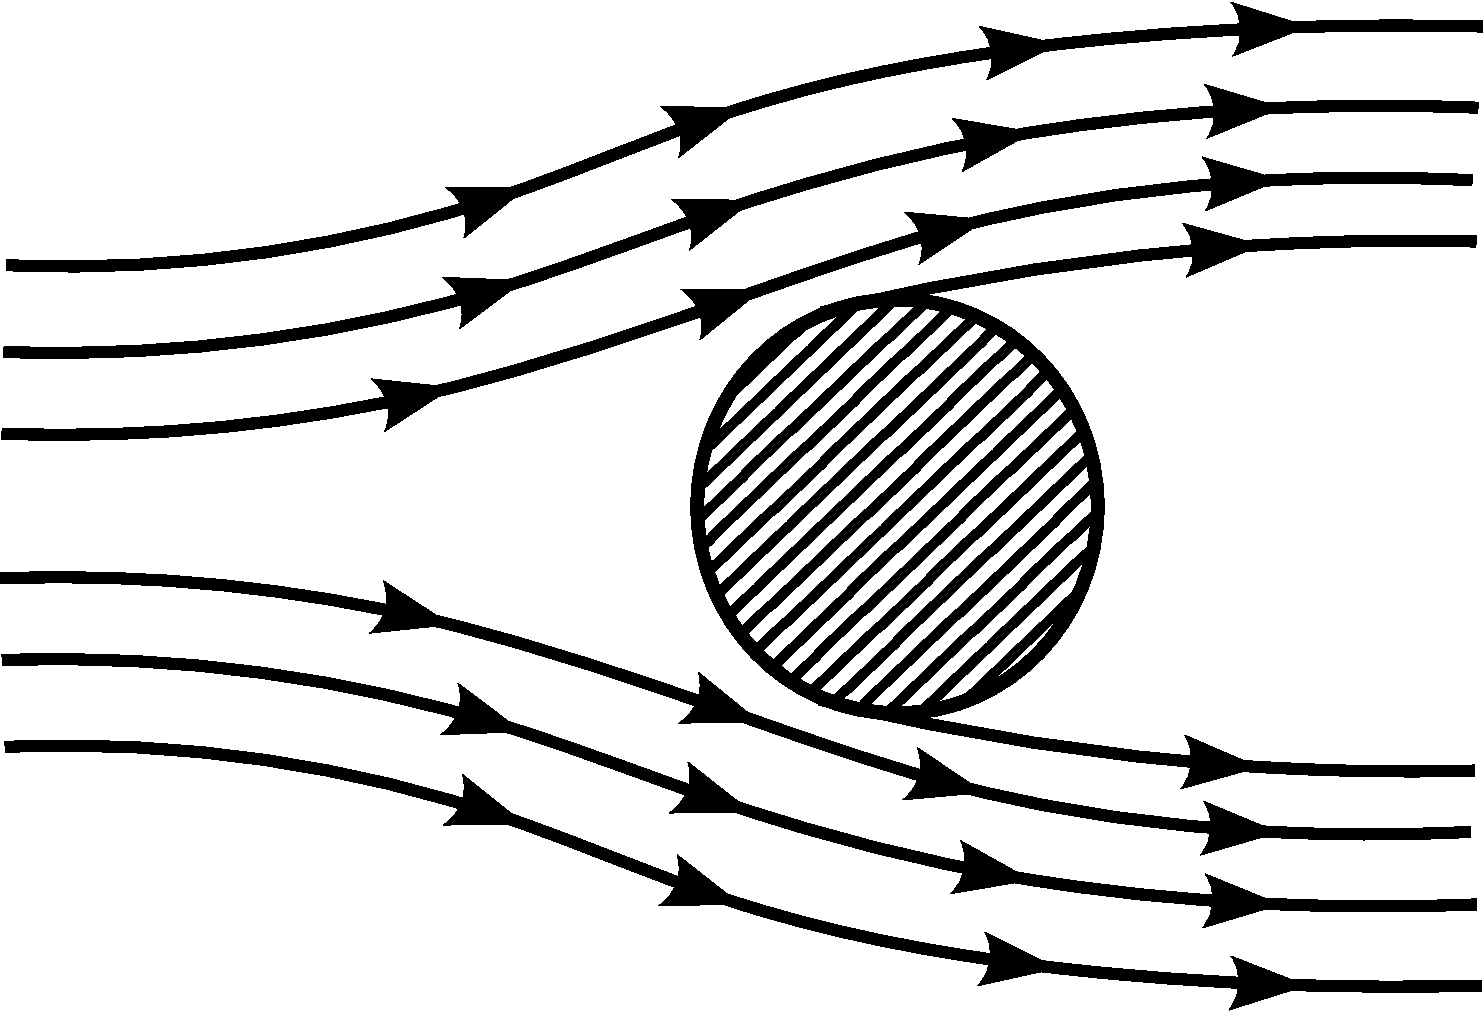
\includegraphics[width=6cm]{fig1}
  \caption{обтекание с поверхностью разрыва}
  \label{fig:f1}
\end{wrapfigure}

Аналогичным образом из закона сохранения циркуляции скорости можно было бы
сделать еще и следующий вывод. Предположим, что в некоторый момент времени
движение жидкости (во всем ее объеме) потенциально. Тогда циркуляция скорости по
любому замкнутому контуру в ней равна нулю \footnote{Для простоты мы считаем здесь,
что жидкость заполняет односвязную область пространства. Для могосвязной области
получился бы тот же самый конечный результат, но при рассуждениях надо было бы делать
специальные оговорки по поводу выбора контуров}. В силу теоремы Томсона можно было бы
заключить, что это будет иметь место и в течение всего дальнейшего времени, т.
е. мы получили бы результат, что если движение жидкости потенциально в некоторый
момент времени, то оно будет потенциальным и в дальнейшем (в частности, должно
было бы быть потенциальным всякое движение, при котором в начальный момент
времени жидкость вообще покоилась). Этому соответствует и тот факт, что
уравнение (\ref{eq:2.11}) удовлетворяется при $\rot\vv = 0$ тождественно.


В действительности, однако, все эти заключения имеют лишь весьма ограниченную
применимость. Дело в том, что приведенное выше доказательство сохранения
равенства $\rot\vv = 0$ вдоль линии тока, строго говоря, неприменимо для линии,
проходящей вдоль поверхности обтекаемого жидкостью твердого тела, уже просто
потому, что ввиду наличия стенки нельзя провести в жидкости замкнутый контур,
который охватывал бы собой такую линию тока. С этим обстоятельством связан тот
факт, что уравнения движения идеальной жидкости допускают решения, в которых на
поверхности обтекаемого жидкостью твердого тела происходит, как говорят, "отрыв
струй": линии тока, следовавшие вдоль поверхности, в некотором месте
"отрываются" от нее, уходя в глубь жидкости. В результате возникает картина
течения, характеризующаяся наличием отходящей от тела "поверхности
тангенциального разрыва", на которой скорость жидкости (будучи направлена в
каждой точке по касательной к поверхности) терпит разрыв непрерывности. Другими
словами, вдоль этой поверхности один слой жидкости как бы скользит по другому
(на Рис \ref{fig:f1} изображено обтекание с поверхностью разрыва, отделяющей движущуюся
жидкость от образующейся позади тела "застойной" области неподвижной жидкости).
С математической точки зрения скачок тангенциальной составляющей скорости
представляет собой, как известно, поверхностный ротор скорости.

При учете таких разрывных течений решение уравнений идеальной жидкости не
однозначно: наряду с непрерывным решением они допускают также и бесчисленное
множество решений с поверхностями тангенциальных разрывов, отходящими от любой
наперед заданной линии на поверхности обтекаемого тела. Подчеркнем, однако, что
все эти разрывные решения не имеют, физического смысла, так как тангенциальные
разрывы абсолютно неустойчивы, в результате чего движение жидкости становится в
действительности турбулентным (см.об этом в гл. III).

Реальная физическая задача об обтекании заданного тела, разумеется, однозначна.
Дело в том, что в действительности не существует строго идеальных жидкостей;
всякая реальная жидкость обладает какой-то, хотя бы и малой, вязкостью. Эта
вязкость может практически совсем не проявляться при движении жидкости почти во
всем пространстве, но сколь бы она ни была мала, она будет играть существенную
роль в тонком пристеночном слое жидкости. Именно свойства движения в этом (так
называемом пограничном) слое и определят в действительности выбор одного из
бесчисленного множества решений уравнений движения идеальной жидкости. При этом
оказывается, что в общем случае обтекания тел произвольной формы отбираются
именно решения с отрывом струй (что фактически приводит к возникновению
турбулентности).

Несмотря на все изложенное, изучение решений уравнений движения, соответствующих
непрерывному стационарному потенциальному обтеканию тел, имеет в некоторых
случаях смысл. Между тем как в общем случае обтекания тел произвольной формы
истинная картина течения практически ничего общего с картиной потенциального
обтекания не имеет, в случае тел, имеющих некоторую особую ("хорошо обтекаемую",
см. \S46). форму, движение жидкости может очень мало отличаться от
потенциального (точнее, оно будет не потенциальным лишь в тонком слое жидкости
вблизи поверхности тела и в сравнительно узкой области "следа" позади тела).

Другим важным случаем, когда осуществляется потенциальное обтекание, являются
малые колебания погруженного в жидкость тела. Легко показать, что если амплитуда
$a$ колебаний мала по сравнению с линейными размерами $l$ тела ($a\ll l$), то
движение жидкости вокруг тела будет всегда потенциальным. Для этого оценим
порядок величины различных членов в уравнении Эйлера
\[
   \pd{\vv}{t}+\vnv = - \nabla w
\]

Скорость у испытывает заметное изменение (порядка скорости $u$ колеблющегося
тела) на протяжении расстояний порядка размеров тела $l$. Поэтому производные от
$\vv$ по координатам — порядка величины $u/l$. Порядок же величины самой
скорости $\vv$ определяется (на не слишком болъших расстояниях от тела)
скоростью $u$. Таким образом, имеем $\vnv \sim u^2/l$. Производная же
$\partial{\vv}/\partial{t}$ — порядка величины $\omega u$, где $\omega$ -
частота колебаний. Поскольку ($\omega \sim u/a$, то имеем $\partial \vv/\partial
t \sim u^2/a$. Из $a \ll l$ следует теперь, что член $\vnv$ мал по сравнению с
$\partial \vv/\partial t$ и может быть опущен, так что уравнение движения
жидкости приобретает вид $\partial \vv/\partial t = - \nabla w$. Применив к
обеим сторонам этого уравнения операцию $\rot$, получаем:
\[
   \pdt \rot \vv = 0,
\]
откуда $\rot \vv = \const$. Но при колебательном движении среднее (по времени)
значение скорости равно нулю; поэтому из $\rot\vv = \const$ следует, $\rot\vv =
0$. Таким образом, движение жидкости, совершающей малые колебания, является (в
первом приближении) потенциальным.

Выясним теперь некоторые общие свойства потенциального движения жидкости. Прежде
всего напомним, что вывод закона сохранения циркуляции, а с ним и всех
дальнейших следствий, был основан на предположении об изэнтропичности течения.
Если же движение не изэнтропично, то этот закон не имеет места; поэтому, даже
если в некоторый момент времени движение является потенциальным, то в
дальнейшем, вообще говоря, завихренность все же появится. Таким образом,
фактически потенциальным может быть лишь изэнтропическое движение.

При потенциальном движении жидкости циркуляция скорости по любому замкнутому
контуру равна нулю:
\begin{equation}
   \label{eq:9.1}
   \oint \vv\;d\vect l = \int \rot \vv \; \df = 0
\end{equation}
Из этого обстоятельства следует, в частности, что при потенциальном течении не
могут существовать замкнутые линии тока \footnote{Этот результат, как и (\ref{eq:9.1}),
может не иметь места при движении жидкости в многосвязной области пространства.
При потенциальном течении в такой области циркуляция скорости может быть отличной
от нуля, если замкнутый контур, вдоль которого она берется, не может быть стянута
в точку так, чтобы нигде не пересечь границ области.}. Действительно, поскольку направление
линии тока совпадает в каждой точке с направлением скорости, циркуляция скорости
вдоль такой линии во всяком случае была бы отличной от нуля.

При вихревом же движении циркуляция скорости, вообще говоря, отлична от нуля. В
этом случае могут существовать замкнутые линии тока; надо, впрочем, подчеркнуть,
что наличие замкнутых линий тока отнюдь не является необходимым свойством
вихревого движения.

Как и всякое векторное поле с равным нулю ротором, скорость потенциально
движущейся жидкости может быть выражена в виде градиента от некоторого скаляра.
Этот скаляр называется \textit{потенциалом скорости}; мы будем обозначать его
посредством $\varphi$:
\begin{equation}
   \label{eq:9.2}
   \vv = \grad \varphi
\end{equation}
Написав уравнение Эйлера в виде (\ref{eq:2.10})
\[
   \pd{\vv}{t} + \frac{1}{2}\nabla v^2 - \vrv = - \nabla w
\]
и подставив в него $\vv = \nabla \varphi$, получаем:
\[
   \grad \left( \pd{\varphi}{t} + \frac{v^2}{2} + w \right) = 0,
\]
откуда находим следующее равенство:
\begin{equation}
   \label{eq:9.3}
   \pd{\varphi}{t} + \frac{v^2}{2} + w = f(t),
\end{equation}
где $f(t)$ - произвольная функция времени. Это равенство представляет собой
первый интеграл уравнений потенциального движения. Функция $f(t)$ в равенстве
(\ref{eq:9.3}) может быть без ограничения общности положена равной нулю за счет
неоднозначности в определении потенциала: поскольку скорость определяется
производными от $\varphi$ по координатам, можно прибавить к $\varphi$ любую
функцию времени.

При стационарном движении имеем (выбирая потенциал $\varphi$ не зависящим от
времени) $\partial\varphi/\partial t=0,\; f(t)=\const$, и (\ref{eq:9.3}) переходит в
уравнение Бернулли
\begin{equation}
   \label{eq:9.4}
   \frac{v^2}{2} + w = \const.
\end{equation}
Необходимо подчеркнуть здесь следующее существенное отличие между уравнениями
Бернулли в случае потенциального и непотенциального движений. В общем случае
произвольного движения const в правой части этого уравнения есть величина,
постоянная вдоль каждой данной линии тока, но, вообще говоря, различная для
разных линий тока. При потенциальном же движении const в уравнении Бернулли есть
величина, постоянная во всем объеме жидкости. Это обстоятельство в особенности
повышает роль уравнения Бернулли при исследовании потенциального движения.

